\section{Architettura}

\begin{figure}[ht]
	\centering
	\includegraphics[width=\textwidth]{Architettura}
	\caption{Architettura del software}
	\label{fig:architecture}
\end{figure}

Il nostro software si compone di tre nodi:
\begin{itemize}
    \item Un nodo che implementa il servizio di object detection, che riceve in input un’immagine da analizzare e, per ogni oggetto nell’immagine, restituisce il relativo bounding box, la classe ed il livello di confidenza relativo alla predizione.
    \item Un nodo che implementa tre servizi che forniscono un’interfaccia verso le funzionalità di text to speech, gestione della posa e movimento della testa di Pepper.
    \item Un nodo master che implementa la funzionalità richiesta dall’homework acquisendo le immagini dal topic della camera di Pepper e utilizzando i servizi offerti dagli altri due nodi.
\end{itemize}
Per l’interfacciamento da e verso Pepper viene utilizzato il NaoQi SDK.

Qua parliamo anche del meccanismo scelto di comunicazione tra i nodi.


\subsection{Server di Object Detection}

Come anticipato, uno dei tre nodi principali del sistema si occupa di esporre un servizio di object detection. 
Questo servizio è implementato attraverso una classe chiamata \verb|PepperObjectDetectorService|, il cui diagramma UML (semplificato) è riportato in figura~\ref{fig:detector_uml}.

\begin{figure}[ht]
	\centering
	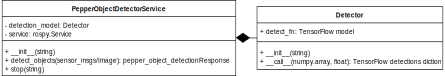
\includegraphics[width=\textwidth]{DetectorUml}
	\caption{Diagramma UML (semplificato) classe \texttt{PepperObjectDetectorService}}
	\label{fig:detector_uml}
\end{figure}

Nel costruttore della classe viene inizializzato il servizio ROS, al quale viene associato come handler il metodo \verb|detect_objects|, e viene inoltre creato un oggetto del tipo \verb|Detector|, che carica il modello di object detection dal percorso fornito e lo esegue sugli input che gli vengono sottomessi tramite chiamata. Il \verb|Detector| viene utilizzato in \verb|detect_objects| per eseguire la detection sugli input inviati al servizio.

Quando il nodo server viene eseguito, viene istanziato un oggetto del tipo 
\verb|PepperObjectDetectorService|, ed il suo metodo \verb|stop| viene registrato per l'esecuzione al momento dello shutdown del nodo, in modo tale che il servizio venga stoppato quando l'esecuzione del server termina. 
Infine il nodo entra in \verb|spin|, in modo da restare in ascolto delle richieste all'object detector.

\subsection{Server di interfaccia verso Pepper}

\subsection{Nodo Master}

Il nodo Master (come \emph{puppet master}, ossia il burattinaio) è stato concepito come il pezzo centrale della nostra applicazione. Questo nodo si interfaccia con tutti i nodi dell'architettura, ed esegue i passi chiave del task in maniera sequenziale. La sequenza di passi è strettamente legata al task, e risulta molto semplice implementare un nuovo nodo che lo sostituisca per personalizzare o modificare i passi, compatibilmente con le interfacce che sono a disposizione nella nostra architettura.

Abbiamo scelto l'approccio sequenziale per semplicità di implementazione. Ciò non toglie che alcune delle azioni possano ottimizzate tramite parallelismi e sincronizzazioni, ma è stato scelto di posticipare questi miglioramenti per dare precedenza al funzionamento completo del sistema secondo le specifiche.

Qui presentiamo la sequenza di operazioni che compie il nodo.
% FRASE DI INIZIO DELLE FASI
\begin{enumerate}
	\item Aspetta che tutti i servizi siano online prima di poter proseguire.
	\item Porta il robot in una posizione neutra con il servizio \verb|pepper_pose| del nodo interfaccia. 
	\item Fa muovere la testa al robot in alcune posizioni predefinite, in cui verrà ``scattata'' una fotografia. Utilizza il servizio \verb|pepper_head_mover| per passare delle traiettorie con posizione singola, visto che dovrà aspettare una immagine dal topic della camera del robot. Nell'attuale implementazione, vengono assunte dieci posizioni che dividono la vista del robot in una matrice $5 \times 2$, in modo che le immagini risultanti siano leggermente sovrapposte.
	\item Esegue lo stitching delle immagini catturate con la libreria OpenCV, ottenendo così un'immagine panoramica di tutta la scena.
	\item Richiede al servizio \verb|pepper_object_detection| gli oggetti presenti nell'immagine panoramica.
	\item Genera una frase per il robot, dividendo gli oggetti trovati tra sinistra, centro e destra, che viene poi inviata al servizio \verb|pepper_tts| per essere riprodotta.
\end{enumerate}

\begin{figure}
	\centering
	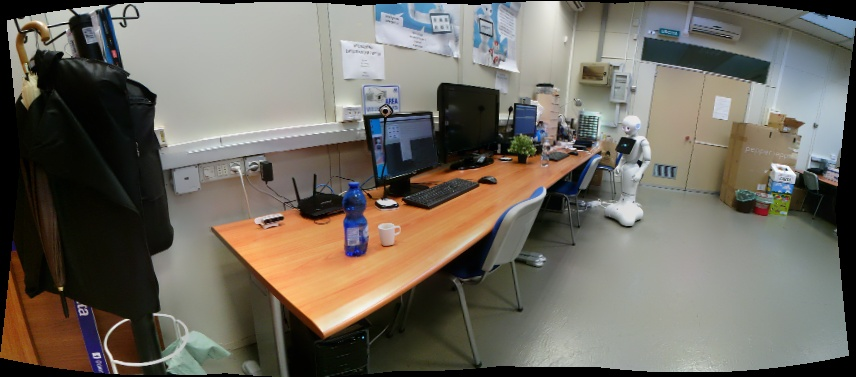
\includegraphics[width=\textwidth]{panorama}
	\caption{Vista del robot dopo l'image stitching.}\label{fig:panorama}
\end{figure}

Una scelta chiave che abbiamo preso è stata quella di eseguire uno stitching sulle immagini della vista (figura~\ref{fig:panorama}). I vantaggi di questo approccio sono molteplici: \begin{enumerate*}[label={(\arabic*)}] \item siamo in grado rilevare efficacemente oggetti che occupano uno spazio che vada oltre la singola immagine (es.\@: un tavolo); \item siamo in grado di evitare che oggetti piccoli divisi su più immagini vengano rilevati più volte, o nessuna; \item permette di allargare il campo visivo a piacere, aggiungendo più catture sia in orizzontale che in verticale.\end{enumerate*} Utilizzando altri approcci, alcune di queste proprietà sarebbero state sostanzialmente più complicate da implementare, e molto probabilmente non avrebbero avuto la stessa robustezza.

Avere una sola immagine fa sì che il detector lavori una sola volta. Se ciò sia effettivamente vantaggioso rispetto ad effettuare la detection su più immagini separate dipende da due fattori: il numero di immagini su cui fare la detection e il modello utilizzato. Nel caso di più immagini potrebbe bastare un detector leggero, visto che queste sono piccole e gli oggetti sono di meno e occupano gran parte della scena. Nel nostro caso, invece, l'immagine risulterà più grande, e soprattutto conterrà più oggetti che occuperanno, relativamente alle dimensioni, meno spazio. Come vedremo nel prossimo paragrafo, sarà necessaria una rete più precisa, soprattutto nel localizzare oggetti piccoli.